\chapter{Experiments and results}
Theory shows that internal agent state transparency and the anti-entropy mechanism reward honesty
and punish any strategic manipulation. We implemented this mechanism and establish in this chapter
how it handles strategic manipulation. More specifically we emulate honest agents and multiple 
types of strategic manipulators in small scale experiments. We can observe the behavior of the 
honest agents and find that strategic manipulators are detected and isolated. We show that honest agents who
execute our mechanism are able to effectively detect malicious agents that do not share or do not verify their partners 
and ignore them for future interactions.

The rest of the chapter is structured as follows: we first give an overview of the software 
architecture. Then we explain the setup of the experiments and the types of strategic manipulation
that will be emulated. Finally we present the results of the experiments.

% In the previous chapters we have explored the problem of dissemination of information in distributed
% trust systems. We offered a solution in the form of our multichain based TrustChain architecture, extended 
% it with internal agent state transparency and designed a mechanism that prevents any free-riding on
% dissemination and validation of information on transactions. In this chapter we aim to prove the 
% properties of the mechanism and architecture by experimental analysis. We built a proof-of-concept
% software that fully implements the architecture and mechanism described in this work. It allows us 
% to run an emulation of an agent network and study the behavior of agents in the presence of strategic
% manipulators.

\section{Experiment design}
The goal of the experiments is to prove the true effectiveness of the mechanism at detecting 
manipulation attempts and isolating malicious agents. Three different types of dishonest behavior 
will be analyzed in the experiments.

\begin{itemize}
    \item \textbf{Dissemination free-rider}: An agent that performs transactions normally but does
    not respond to exchange requests or start own exchanges.
    \item \textbf{Validation free-rider}: An agent that performs exchanges and transactions normally
    but does not perform any validation
    \item \textbf{Forking}: An agent creates two conflicting transactions and forwards them to two 
    different partners without telling them about the other transaction.  
\end{itemize}

% The goal of the experimental analysis is to show that free-riding on dissemination and validation of
% transaction information is no longer possible with the extension of TrustChain proposed in 
% chapter~\ref{chap:state_transparency} and the mechanism in chapter~\ref{chap:mechanism}. This would
% be a major step towards a secure and valid distributed trust system. 

In the experiments we emulate small agent networks up to 6 agents. We assume that agents are trying to perform 
interactions with each other. The experiments are not concerned with the actual trust agents have 
in each other so we keep transaction blocks empty. Agents are acting completely autonomously 
but knows about all the other agents in the network. At a frequency of 20 per second agents go through
rounds, in each round an agent has a 1\% chance of starting an interaction. This adds up to approximately
1 transaction every 5 seconds. In addition agents respond to interaction requests from their peers 
asynchronously. At the start of the interaction a peer is selected with uniform probability. If an
interaction with the selected partner is already ongoing, the new interaction request is cancelled
without selecting a new partner. The same happens when the selected partner is a known malicious 
agent. Once the interaction is started honest agents perform according the mechanism as described in
chapter \ref{chap:mechanism}. The other types of agents each have some deviation from the expected
behavior in order to obtain an unfair advantage.

\begin{itemize}
    \item \textbf{Dissemination free-rider}: An agent that performs transactions normally but does
    not respond to exchange requests or start own exchanges.
    \item \textbf{Validation free-rider}: An agent that performs exchanges and transactions normally
    but does not perform any validation
\end{itemize}

With these types of agent we run experiments with different sets of agents. In experiments with only
a single dishonest agent, the experiment is successful if the honest agents stay among themselves
and ignore the dishonest agent. That is, the dishonest agent should have 0 transactions at the end
of the experiment. In the case with multiple dishonest agents we have to make a distinction between
multiple single acting dishonest agents and collaborating groups of dishonest agents. 

\section{Implementation details}

\begin{itemize}
    \item Python implementation 
    \item zermq sockets
\end{itemize}


\section{Experiment results}
\subsection{Dissemination free-riders}
\begin{figure}
    \begin{subfigure}{\textwidth}
      \centering
      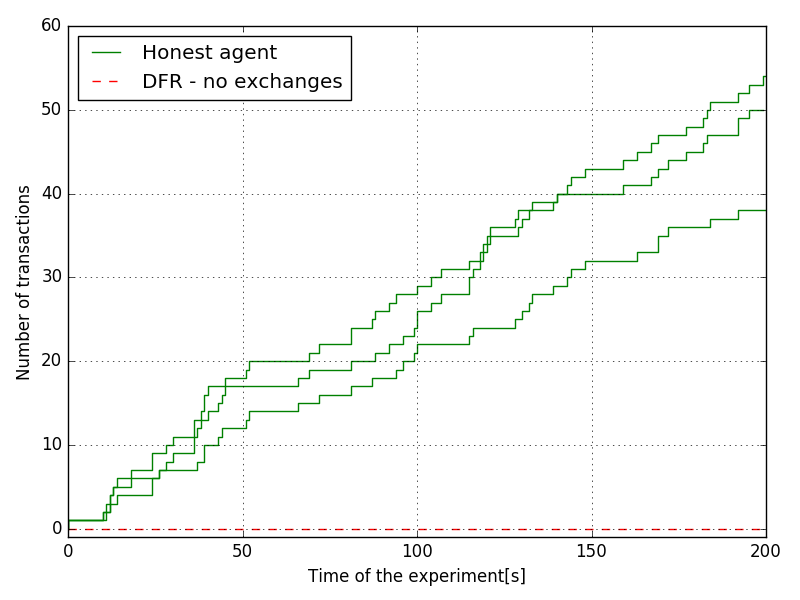
\includegraphics[width=.6\linewidth]{images/DFR_no_exchanges}
      \caption{Transactions over time of honest agents with dissemination free-rider that does not 
      perform any exchanges}
      \label{fig:DFR_no_exchanges}
    \end{subfigure}\\
    \begin{subfigure}{\textwidth}
      \centering
      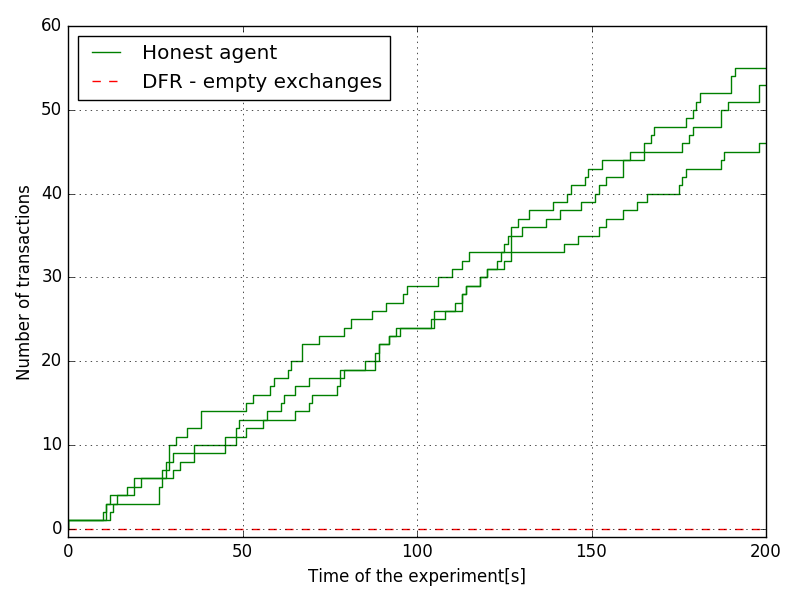
\includegraphics[width=.6\linewidth]{images/DFR_empty_exchanges}
      \caption{Transactions over time of honest agents with dissemination free-rider that creates 
      empty exchanges}
      \label{fig:DFR_empty_exchanges}
    \end{subfigure}\\
    \begin{subfigure}{\textwidth}
        \centering
        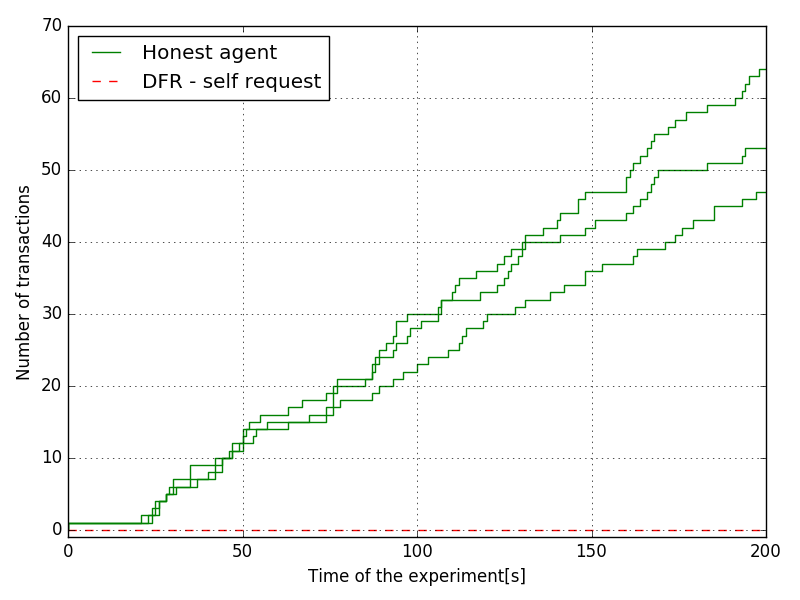
\includegraphics[width=.6\linewidth]{images/DFR_self_request}
        \caption{Transactions over time of honest agents with dissemination free-rider that only 
        exchanges own data}
        \label{fig:DFR_self_request}
      \end{subfigure}
\end{figure}

\subsection{Collaborating dissemination free-riders}

\begin{figure}[h!]
    \centering
    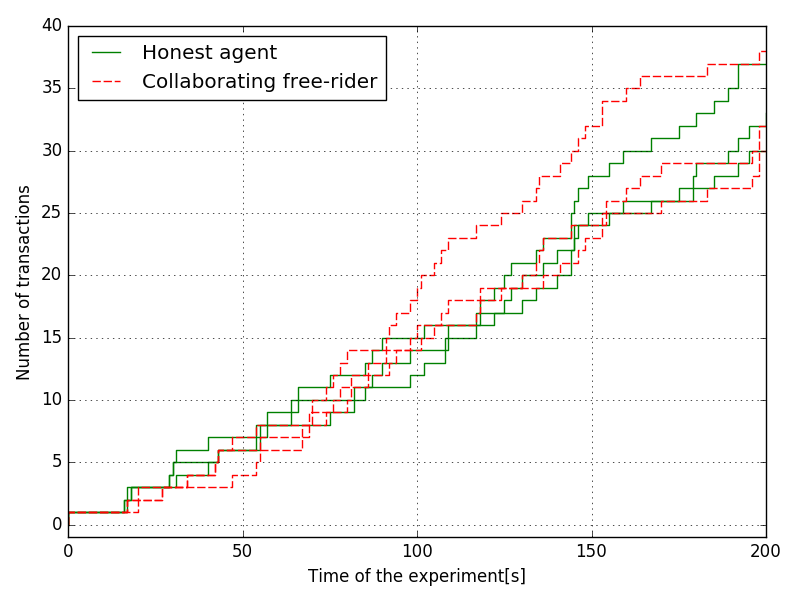
\includegraphics[width=0.7\textwidth]{images/50percent}
    \caption{Transaction history of three honest agents and three dissemination free-riders
    that are cooperating}
    \label{fig:50percent}
\end{figure}

\begin{figure}[h!]
    \centering
    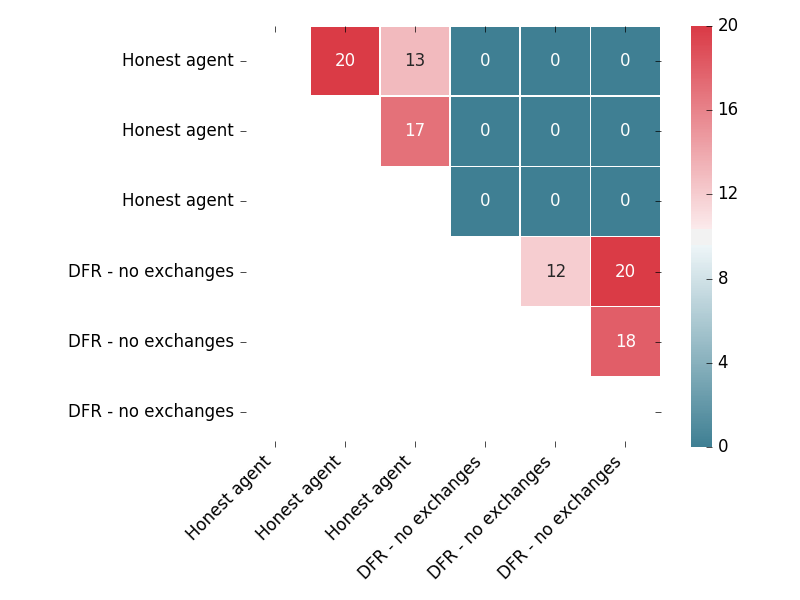
\includegraphics[width=0.7\textwidth]{images/50percent_interaction_matrix}
    \caption{Interaction matrix of three honest agents and three dissemination free-riders who are cooperating}
    \label{fig:50percent}
\end{figure}

\subsection{Malicious behavior}

\begin{figure}
    \begin{subfigure}{\textwidth}
      \centering
      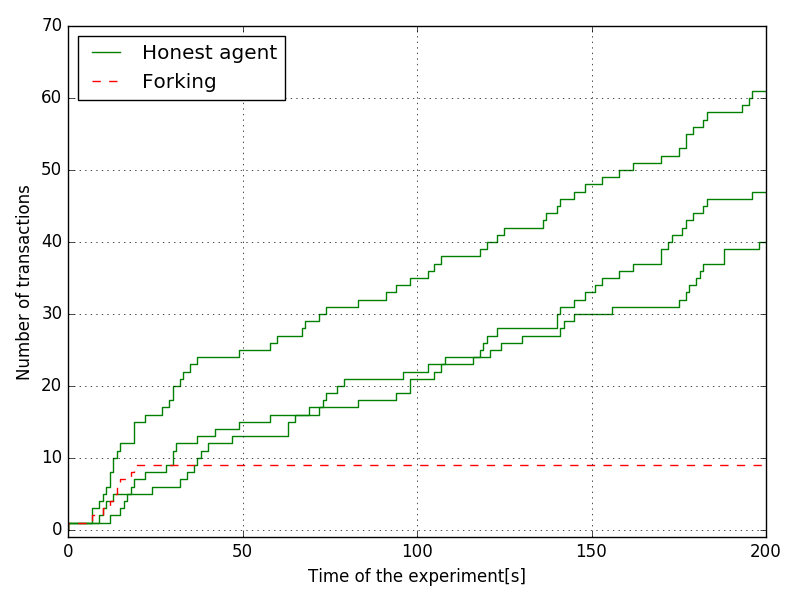
\includegraphics[width=.6\linewidth]{images/forking}
      \caption{Transaction history of three honest agents interacting with one strategic manipulator who performs a fork}
      \label{fig:forking}
    \end{subfigure}\\
    \begin{subfigure}{\textwidth}
      \centering
      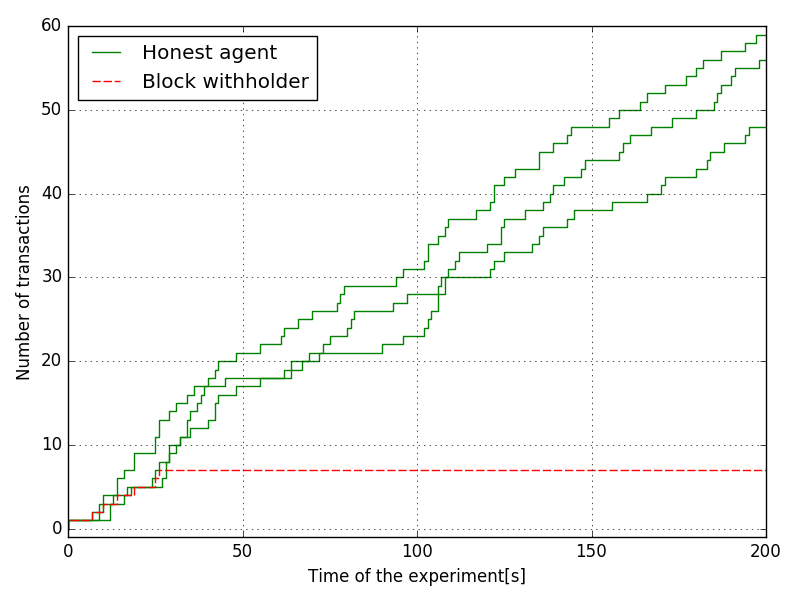
\includegraphics[width=.6\linewidth]{images/transaction_hiding}
      \caption{Transactions over time of three honest agents with one strategic manipulator who tries to hide a transaction}
      \label{fig:DFR_empty_exchanges}
    \end{subfigure}\\
\end{figure}

\subsection{Verification free-rider}

\begin{figure}
    \begin{subfigure}{\textwidth}
      \centering
      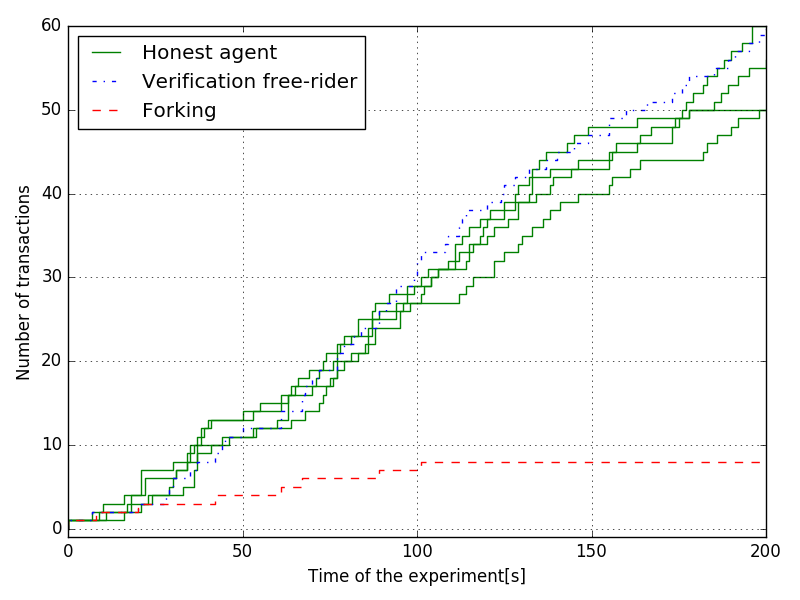
\includegraphics[width=.6\linewidth]{images/verification_doublespend_honest}
      \caption{Transaction history of three honest agents interacting with one strategic manipulator who performs a fork and a verification free-rider}
      \label{fig:verification_doublespend_honest}
    \end{subfigure}\\
    \begin{subfigure}{\textwidth}
      \centering
      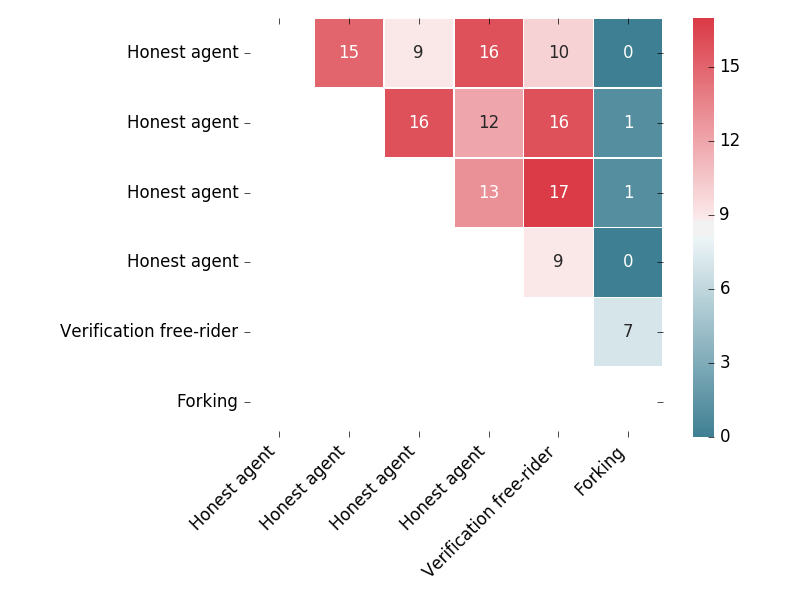
\includegraphics[width=.6\linewidth]{images/verification_doublespend_honest_matrix}
      \caption{Interaction matrix of three honest agents with one strategic manipulator who performs a fork and a verification free-rider}
      \label{fig:verification_doublespend_honest_matrix}
    \end{subfigure}\\
\end{figure}

\begin{figure}
    \begin{subfigure}{\textwidth}
      \centering
      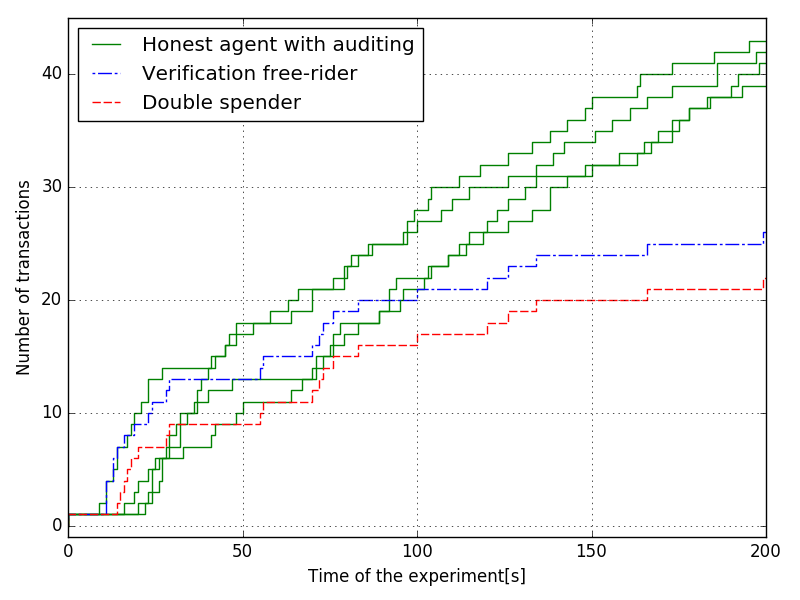
\includegraphics[width=.6\linewidth]{images/verification_doublespending}
      \caption{Transaction history of three honest agents with replay verification interacting with one strategic manipulator who performs a fork and a verification free-rider}
      \label{fig:verification_doublespending}
    \end{subfigure}\\
    \begin{subfigure}{\textwidth}
      \centering
      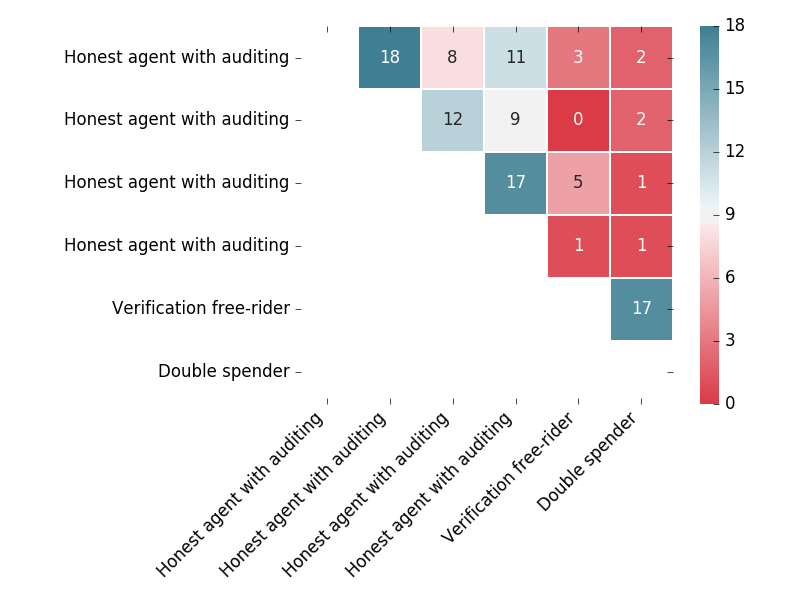
\includegraphics[width=.6\linewidth]{images/verification_doublespending_matrix}
      \caption{Interaction matrix of three honest agents with replay verification with one strategic manipulator who performs a fork and a verification free-rider}
      \label{fig:verification_doublespending_matrix}
    \end{subfigure}\\
\end{figure}

\section{}

\subsection{Sybil attack}